Another method to handle data acquisition and memory storage is through the Streaming application, which enables input data to be streamed from the Red Pitaya to a file saved on the system's SD card or on a remote computer via the ethernet protocol. Figure \ref{fig:ch2_stream_old} shows a screenshot of the application's web interface, where various configurations can be set, including sampling frequency, input channel selection, input resolution and attenuation, calibration, etc. The data can be saved as the following types: \textit{.wav}, \textit{.tdms}, or \textit{.bin}.

\begin{figure}[ht]
    \centering
    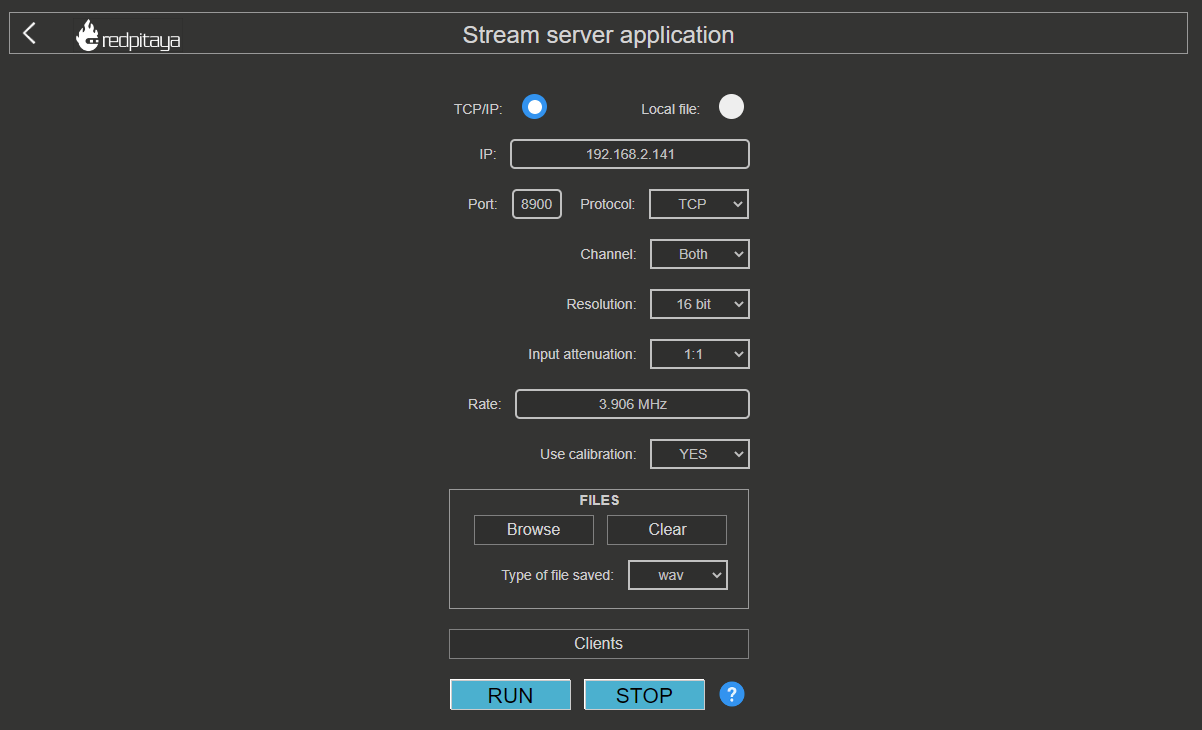
\includegraphics[width=0.9\columnwidth]{images/chapter_2/2_stream/stream_old.png}
    \caption{Web interface of the Streaming application that comes with the Red Pitaya.}
    \label{fig:ch2_stream_old}
\end{figure}

At first glance, the features that come with the Streaming application make it a good candidate for acquiring analog input data. So then it was necessary to discover its mechanism with respect to RAM storage, in order to modify the memory space to acquire sufficient amount of data at once to meet the experimental requirement represented in Equation \eqref{eq:rp_memory}.

%%%%%%%%%%%%%%%%%%%%%%%%%%%%%%%%%%%%%%%%%%%%%%%%%%%%%%%%%%%%%%%%%%%%%%%%%%%%%%%%

\paragraph{Tests}

To familiarize with how the Streaming server works, I started with some sampling tests. First we assume that the application, similar to the oscilloscope, is allotted 16$^4$ = 65,536 bytes of memory space per channel by default. Sampling at 16 bits per sample, this corresponds to 32,768 samples that can be stored at once. At the maximum sampling rate of 125 MHz, one period of input signal at $f_\text{full} = 3815$ Hz will fully occupy this amount of memory space. Using these parameters, input signal data with RAW units were streamed and saved to a \textit{.bin} file to be processed and evaluated.

%%%%%%%%%%%%%%%%%%%%%%%%%%%%%%%%%%%%%%%%%%%%%%%%%%%%%%%%%%%%%%%%%%%%%%%%%%%%%%%%

\begin{figure}[ht]
    \centering
    \begin{subfigure}[t]{0.47\linewidth}
        \centering
        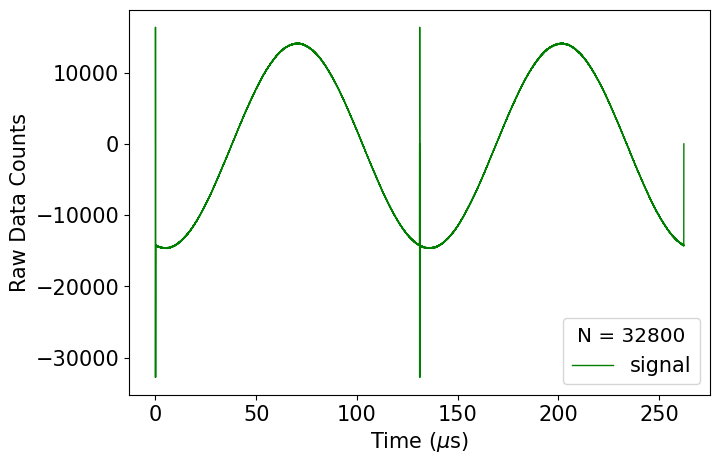
\includegraphics[width=\textwidth]{images/chapter_2/2_stream/stream_3815Hz.png}
        \caption{}
        \label{fig:ch2_stream_3815Hz}
    \end{subfigure}
    \hspace{.025\linewidth}
    \begin{subfigure}[t]{0.47\linewidth}
        \centering
        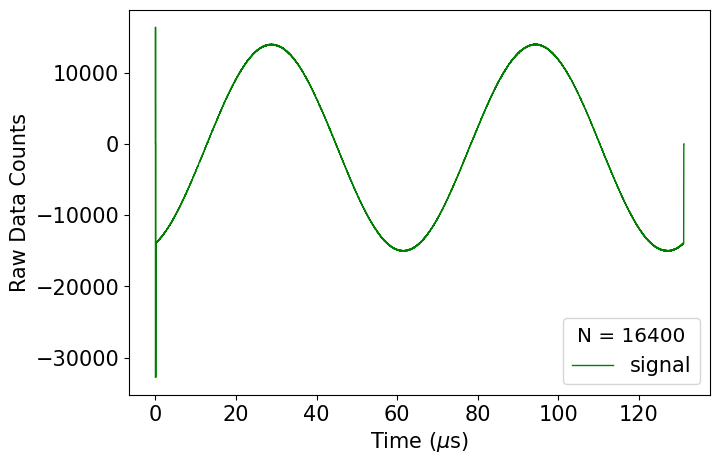
\includegraphics[width=\textwidth]{images/chapter_2/2_stream/stream_7629Hz.png}
        \caption{}
        \label{fig:ch2_stream_7629Hz}
    \end{subfigure}
    \caption{Input signal data streamed from the Streaming application for (a) original and (b) extended allotted system memory space for signal data storage.}
    \label{fig:ch2_lipid_og_ex}
\end{figure}

\paragraph{Results}

Figure \ref{fig:ch2_stream_3815Hz} shows the streamed signal data plotted with respect to the expected time span. Immediately, we recognize that the actual number of samples taken is greater than the input configuration, as if this number is rounded up to the nearest hundred, which is an unexpected and undesired behavior. Additionally, we see sharp lines at the beginning, middle, and end of the signal, which we hypothesized as indications of memory overflow. These lines imply that the memory space allotted to the Streaming app is actually half the amount predicted, at 16$^4$/2 = 32,768 bytes or roughly 16,400 samples. Since exactly one period of the signal with $f_\text{full} = 3815$ Hz is contained in the ``halved" memory space, referring to Equation \eqref{eq:f_full}, it must mean that the sampling rate was actually not 125 MHz, as entered on the application web interface, but half of that rate. This is another unexpected and undesired behavior of the Streaming application.

Another test was done using 16,384 samples as the maximum sample count that can be stored in the allotted memory space, which at 125 MHz sampling speed (entered on the application web interface), corresponds to $f_\text{full}$ = 7629 Hz. The signal data plot is shown in Figure \ref{fig:ch2_stream_7629Hz}. The absence of a sharp middle line indicates that memory overflow did not occur, and the fact that 2 signal periods where captured confirms that the actual sample rate was indeed half of what was entered, validating our assumptions and hypothesis from the previous test run.

%%%%%%%%%%%%%%%%%%%%%%%%%%%%%%%%%%%%%%%%%%%%%%%%%%%%%%%%%%%%%%%%%%%%%%%%%%%%%%%%

\paragraph{Conclusion}

A deeper investigation into the Streaming application's sampling rate setting reveals that only certain number values are accepted by the application. I then explored the front-end Javascript code associated with this input field and found numerous strange bugs. We hoped that upgrading the Red Pitaya ecosystem from the current 1.04 version to the newest 2.03 version will introduce fixes to the Streaming app, for both the sampling count and sampling rate fields. Unfortunately, this was not the case, as the same issues remain in ecosystem 2.03. We determined that it was not worth the effort trying to debug the Streaming application, so we decided to move onto another alternative method for data acquisition for analog inputs.